\documentclass[aspectratio=169,11pt]{beamer}
\usepackage[T1]{fontenc}
\usepackage{newtxtext,newtxmath}
\usepackage{tikz,pgfplots}
\pgfplotsset{compat=1.17}
\usetikzlibrary{arrows.meta,positioning,shapes.geometric}
\usepackage{booktabs,tabularx,amsmath}

\definecolor{kuet}{RGB}{0,122,61}
\definecolor{ink}{RGB}{30,40,50}
\usetheme{default}
\usecolortheme{default}
\setbeamercolor{frametitle}{fg=white,bg=kuet}
\setbeamercolor{normal text}{fg=ink}
\setbeamercolor{itemize item}{fg=kuet}
\setbeamercolor{block title}{fg=white,bg=kuet}
\setbeamercolor{block body}{bg=kuet!8}
\setbeamertemplate{navigation symbols}{}
\setbeamertemplate{itemize items}[circle]
\setbeamerfont{frametitle}{series=\bfseries,size=\large}
\setbeamerfont{block title}{size=\small}
\setbeamertemplate{footline}{\hfill\scriptsize\color{gray}Sentinel \quad \insertframenumber/10\hspace{0.6em}\vspace{0.4em}}
\setbeamertemplate{frametitle}{%
  \nointerlineskip\begin{beamercolorbox}[wd=\paperwidth,ht=2.6ex,dp=1.2ex,leftskip=1.2em]{frametitle}\usebeamerfont{frametitle}\insertframetitle\end{beamercolorbox}}
\tikzset{box/.style={draw=kuet,rounded corners=2pt,align=center,font=\scriptsize,inner sep=3pt,fill=white},arr/.style={-{Stealth[length=2mm]},thick,kuet}}
\newcommand{\pic}[2]{\includegraphics[width=#1\linewidth]{images/#2}}

\begin{document}

% 1 ---------------- cover
\begin{frame}[plain]
\begin{tikzpicture}[remember picture,overlay]
  \fill[kuet] (current page.north west) rectangle ([yshift=-3.2cm]current page.north east);
  \node[white,align=center,font=\small] at ([yshift=-0.9cm]current page.north) {Khulna University of Engineering \& Technology\\Department of Computer Science and Engineering};
  \node[white,font=\footnotesize] at ([yshift=-2.5cm]current page.north) {CSE 4102: Computer Graphics and Image Processing Laboratory \,|\, 4th Year 1st Term};
\end{tikzpicture}
\vspace{3.1cm}
\begin{center}
{\fontsize{34}{38}\selectfont\bfseries\color{kuet}Sentinel}\\[4pt]
{\Large\bfseries A Fully Procedural Game Engine\\and Open-World Military Shooter}\\[10pt]
{\small Nothing is loaded from a model, image or sound file: everything is generated from code and a seed.}
\end{center}
\vfill
\begin{columns}[b]
\column{0.4\textwidth}\footnotesize
\textbf{Presented by}\\ Md.\ Shifat Hasan, Roll 2107067
\column{0.3\textwidth}\centering

\includegraphics[height=1.5cm]{images/KUET_Logo.png}
\column{0.3\textwidth}\footnotesize\raggedleft
\textbf{Instructors}\\ Md Tajmilur Rahman\\ Md.\ Mubtashim Abrar Nihal\\[2pt] October 7, 2026
\end{columns}
\end{frame}

% 2 ---------------- outline
\begin{frame}[c]{Outline}
\begin{columns}[T]
\column{0.55\textwidth}
\begin{enumerate}\setlength{\itemsep}{5pt}
  \item Problem and objectives
  \item Engine architecture
  \item Procedural content: shapes and textures
  \item The rendering pipeline
  \item World, physics and gameplay
  \item Results and verification
  \item Challenges, limits and future work
\end{enumerate}
\column{0.42\textwidth}
\pic{1}{showroom.jpg}\\[-1pt]{\scriptsize\centering Every material is a code-generated recipe.}
\end{columns}
\end{frame}

% 3 ---------------- problem
\begin{frame}[c]{1. Problem and objectives}
\begin{columns}[T]
\column{0.55\textwidth}
\textbf{The question:} can a complete, good-looking, playable 3D game be made by \emph{code alone} on a student laptop?
\vspace{4pt}
\vspace{-2pt}\begin{block}{Two hard limits}
\begin{itemize}\setlength{\itemsep}{1pt}
 \item No pre-saved model, image or precomputed data file (only shader text is read)
 \item macOS stops at OpenGL~4.1: no compute shaders
\end{itemize}
\end{block}
\textbf{Objectives}\vspace{-2pt}
\begin{enumerate}\small\setlength{\itemsep}{1pt}
 \item Layered engine, dependencies only downward
 \item All meshes, textures, sounds from code and seeds
 \item Modern renderer: PBR, shadows, sky, post-processing
 \item Playable game: vehicles, ladders, doors, mission
 \item Verified by tests and a 16.7\,ms frame budget
\end{enumerate}
\column{0.43\textwidth}
\pic{1}{base.jpg}\\[4pt]
\pic{0.7}{demo.jpg}
\end{columns}
\end{frame}

% 4 ---------------- architecture
\begin{frame}[c]{2. Engine architecture}
\begin{columns}[T]
\column{0.5\textwidth}
\centering
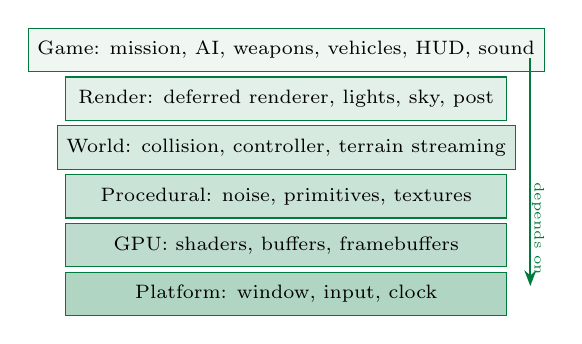
\begin{tikzpicture}
\foreach \i/\t in {0/{Game: mission, AI, weapons, vehicles, HUD, sound},1/{Render: deferred renderer, lights, sky, post},2/{World: collision, controller, terrain streaming},3/{Procedural: noise, primitives, textures},4/{GPU: shaders, buffers, framebuffers},5/{Platform: window, input, clock}}
  \node[draw=kuet,minimum width=5.6cm,minimum height=0.55cm,font=\scriptsize,fill=kuet!\the\numexpr 6+\i*5\relax] at (0,-\i*0.62) {\t};
\draw[arr] (3.1,-0.1)--(3.1,-3.0) node[midway,right,font=\tiny,rotate=-90,yshift=0.1cm]{depends on};
\end{tikzpicture}
\\[4pt]{\footnotesize A lower layer never knows a higher one.}
\column{0.48\textwidth}
\textbf{Readable by design}
\begin{itemize}\setlength{\itemsep}{4pt}
 \item \texttt{Main.odin} = table of contents: init, loop (input, update, render), shutdown
 \item One feature per file; procedures $\approx$40 lines
 \item Content is data: object = table of \emph{part, transform, deformers, material}
 \item Every GL call checked; preconditions asserted
\end{itemize}
\vspace{4pt}
\begin{block}{Size} 164 Odin files ($\approx$19\,200 lines), 47 GLSL files ($\approx$2\,000 lines), 138 commits\end{block}
\end{columns}
\end{frame}

% 5 ---------------- procedural
\begin{frame}{3. Procedural content: shapes and textures}
\begin{columns}[T]
\column{0.56\textwidth}
\pic{1}{noise_stages.png}\\[-2pt]{\scriptsize gradient, fractal, warped, ridged, cellular noise}
\vspace{3pt}
\begin{itemize}\setlength{\itemsep}{3pt}\small
 \item \textbf{Fractal noise} sums octaves, each 2$\times$ finer and $\tfrac12$ as strong; wrapped grid index $\Rightarrow$ \textbf{exact tiling}
 \item 18 recipes $\to$ 22 materials, baked once at 1024$^2$
 \item \textbf{Scharr} filter turns height into bumps
 \item Shapes: primitives + noise deformers; legs by two-bone IK
\end{itemize}
\column{0.42\textwidth}
\begin{block}{Fractal noise}
$\displaystyle F(\mathbf x)=\frac{\sum_{i=0}^{n-1}2^{-i}\nu(2^i\mathbf x)}{\sum_{i=0}^{n-1}2^{-i}}$
\end{block}
\begin{block}{Normal from height}
$\displaystyle h_x\!\approx\!\frac{3(h_{NE}\!+\!h_{SE}\!-\!h_{NW}\!-\!h_{SW})\!+\!10(h_E\!-\!h_W)}{32\Delta N}$\\[1pt]\scriptsize $\hat n\propto(-kh_x,-kh_y,1)$
\end{block}
\begin{block}{Vertex push}
$\mathbf p'=\mathbf p+A\,\nu(f\mathbf p)\,\hat n$, \ $|\mathbf p'-\mathbf p|\le A$
\end{block}

\end{columns}
\end{frame}

% 6 ---------------- rendering
\begin{frame}[c]{4. The rendering pipeline}
\centering
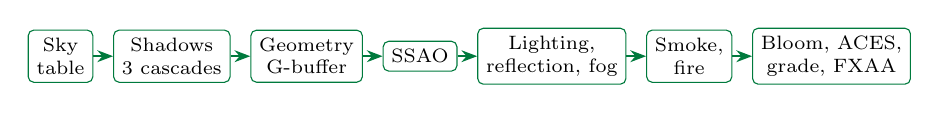
\begin{tikzpicture}[node distance=0.15cm and 0.25cm]
\node[box] (s) {Sky\\table};\node[box,right=of s] (sh) {Shadows\\3 cascades};\node[box,right=of sh] (g) {Geometry\\G-buffer};\node[box,right=of g] (ao) {SSAO};\node[box,right=of ao] (li) {Lighting,\\reflection, fog};\node[box,right=of li] (pa) {Smoke,\\fire};\node[box,right=of pa] (po) {Bloom, ACES,\\grade, FXAA};
\foreach \x/\y in {s/sh,sh/g,g/ao,ao/li,li/pa,pa/po}\draw[arr](\x)--(\y);
\end{tikzpicture}
\vspace{3pt}
\begin{columns}[T]
\column{0.5\textwidth}\raggedright\small
\textbf{Deferred shading:} first store each pixel's colour, normal, shininess, depth (the ``data poster''), then light it once; many lights stay cheap.
\begin{block}{Cook--Torrance reflection}
\scriptsize$f=\frac{(1-F_l)(1-F_v)\mathbf c_d}{\pi}+D\,V\,F$\\
$D=\frac{\alpha^2}{\pi((\mathbf n\cdot\mathbf h)^2(\alpha^2-1)+1)^2}$, \ $F=F_0+(1-F_0)(1-\mathbf v\cdot\mathbf h)^5$
\end{block}
\begin{block}{Fog and tone map}
\scriptsize$C=TC_s+(1-T)C_h,\ T=e^{-kd}$\\ $C_{\rm out}=\frac{x(2.51x+0.03)}{x(2.43x+0.59)+0.14}$
\end{block}
\column{0.48\textwidth}
\pic{1}{dusk.jpg}\\[1pt]{\scriptsize\centering Dusk: sun, sky, haze, shadows, clouds}
\end{columns}
\end{frame}

% 7 ---------------- world
\begin{frame}{5. World, physics and gameplay}
\begin{columns}[T]
\column{0.5\textwidth}\small
\begin{itemize}\setlength{\itemsep}{2.5pt}
 \item \textbf{Sky:} sun height $\sin e=\sin\varphi\sin\delta+\cos\varphi\cos\delta\cos h$; scattering sky; wind-driven cumulus and cirrus: $\mathbf P_{xz}=\frac{H}{d_y}(d_x,d_z)+\mathbf w t$
 \item \textbf{Terrain:} warped ridged noise, 64\,m streamed chunks
 \item \textbf{Trees:} 4 species, per-tree size and tint, cantilever wind sway
 \item \textbf{Vehicles:} jeep, truck, carrier, tank, helicopter; bicycle steering $\dot\psi=\frac{v\tan\delta}{L}$, power fade $\dot v=a_0(1-0.6\frac{|v|}{v_{\max}})$
 \item \textbf{Ladders:} 4-state grip machine, hands on rungs
 \item \textbf{Mission:} hack, destroy, rescue, extract; stealth AI; all sound synthesised
\end{itemize}
\column{0.48\textwidth}
\pic{0.8}{gate_day.jpg}\\[2pt]
\begin{columns}\column{0.5\linewidth}\pic{1}{ladder.jpg}\column{0.5\linewidth}\pic{1}{soldiers.jpg}\end{columns}
\end{columns}
\end{frame}

% 8 ---------------- results
\begin{frame}{6. Results and verification}
\begin{columns}[T]
\column{0.5\textwidth}
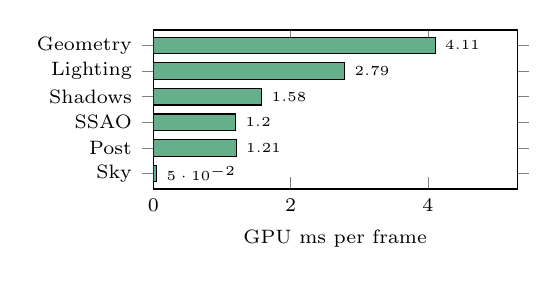
\begin{tikzpicture}
\begin{axis}[xbar,width=6.2cm,height=3.6cm,symbolic y coords={Sky,Post,SSAO,Shadows,Lighting,Geometry},ytick=data,xmin=0,xmax=5.3,scaled x ticks=false,nodes near coords,every node near coord/.append style={font=\tiny},tick label style={font=\scriptsize},xlabel={GPU ms per frame},xlabel style={font=\scriptsize},bar width=6pt,enlarge y limits=0.12]
\addplot[fill=kuet!60] coordinates {(0.05,Sky)(1.21,Post)(1.20,SSAO)(1.58,Shadows)(2.79,Lighting)(4.11,Geometry)};
\end{axis}
\end{tikzpicture}\\[2pt]
{\small \textbf{10.9\,ms} GPU of the 16.7\,ms budget (1080p); display locks 60\,Hz.}
\vspace{4pt}
\begin{tabularx}{\linewidth}{lr}\toprule\multicolumn{2}{l}{\small\textbf{Verification}}\\\midrule
\scriptsize Unit tests (13 packages) & \scriptsize 281\\
\scriptsize TextureCheck (exact tiling) & \scriptsize 8\,318\\
\scriptsize RenderCheck & \scriptsize 318\,567\\
\scriptsize GpuCheck & \scriptsize 30\\
\scriptsize Scripted playthroughs (5/5 objectives) & \scriptsize 2\\\bottomrule\end{tabularx}
\column{0.48\textwidth}
\pic{0.78}{hq.jpg}\\[2pt]
\pic{0.78}{map.jpg}
\end{columns}
\end{frame}

% 9 ---------------- challenges
\begin{frame}[c]{7. Challenge solved, limits and future work}
\begin{columns}[T]
\column{0.58\textwidth}
\large\textbf{Bug: a bright vertical line at night.} Found by bisecting draw items, lights and passes. Cause: the fog colour sampled the \emph{whole} sky, so one horizon star painted a streak down every surface in its column. Fix: fog uses the smooth atmosphere only.
\vspace{3pt}
\begin{columns}\column{0.5\linewidth}\pic{1}{gate_night_bug.jpg}\\[-2pt]{\scriptsize\centering before}\column{0.5\linewidth}\pic{1}{gate_night.jpg}\\[-2pt]{\scriptsize\centering after}\end{columns}
\column{0.4\textwidth}
\begin{block}{Limitations}\footnotesize
Blocky primitive models; no true global illumination; lumpy foliage; tuned by scripts and screenshots, not a big playtest.
\end{block}
\begin{block}{Future work}\footnotesize
Leaf cards, screen-space GI, point-light shadows, multiplayer, a compute-shader port.
\end{block}
\begin{block}{Take-away}\footnotesize
Most ``art'' is a few simple ideas (smooth noise, a lighting formula, transforms) applied consistently and tested.
\end{block}
\end{columns}
\end{frame}

% 10 ---------------- references + thanks
\begin{frame}[c]{References and thank you}
\begin{columns}[T]
\column{0.68\textwidth}\scriptsize\setlength{\parskip}{1pt}
[1] K. Perlin, ``Improving noise,'' \emph{ACM TOG (SIGGRAPH)}, 21(3), 2002.\par
[2] S. Worley, ``A cellular texture basis function,'' \emph{SIGGRAPH}, 1996.\par
[3] R. Cook and K. Torrance, ``A reflectance model for computer graphics,'' \emph{ACM TOG}, 1(1), 1982.\par
[4] B. Walter et al., ``Microfacet models for refraction through rough surfaces,'' \emph{EGSR}, 2007.\par
[5] B. Karis, ``Real shading in Unreal Engine 4,'' SIGGRAPH Course, 2013.\par
[6] S. Hillaire, ``A scalable and production ready sky and atmosphere rendering technique,'' \emph{CGF}, 39(4), 2020.\par
[7] R. Dimitrov, ``Cascaded shadow maps,'' NVIDIA, 2007.\par
[8] M. Oren and S. Nayar, ``Generalization of Lambert's reflectance model,'' \emph{SIGGRAPH}, 1994.\par
[9] K. Narkowicz, ``ACES filmic tone mapping curve,'' 2016.\par
[10] J. Jimenez, ``Next generation post processing in Call of Duty: Advanced Warfare,'' SIGGRAPH, 2014.\par
[11] T. Lottes, ``FXAA,'' NVIDIA, 2009.\par
[12] M. Segal and K. Akeley, \emph{The OpenGL Graphics System, v4.1}, Khronos, 2010.\par
[13] I. Quilez, ``Domain warping,'' iquilezles.org.\par
[14] S. Hargreaves and M. Harris, ``Deferred shading,'' NVIDIA, GDC 2004.\par
[15] H. Scharr, ``Optimal operators in digital image processing,'' Ph.D., Heidelberg, 2000.\par
[16] T. Akenine-M\"oller et al., \emph{Real-Time Rendering}, 4th ed., CRC Press, 2018.
\column{0.3\textwidth}
\centering\vspace{0.6cm}
{\Huge\bfseries\color{kuet}Thank you}\\[8pt]
{\small Questions are welcome}\\[10pt]

\includegraphics[height=1.6cm]{images/KUET_Logo.png}\\[6pt]
{\scriptsize Md.\ Shifat Hasan \,|\, Roll 2107067}
\end{columns}
\end{frame}
\end{document}
